% !TEX program = xelatex
\documentclass[12pt]{exam}

\usepackage{setspace}
\usepackage{listings}
\usepackage{xcolor}
\usepackage{xepersian}
\usepackage{amsmath,amssymb}

% Define colors
\definecolor{codegreen}{rgb}{0,0.6,0}
\definecolor{codegray}{rgb}{0.5,0.5,0.5}
\definecolor{codepurple}{rgb}{0.58,0,0.82}
\definecolor{backcolour}{rgb}{0.95,0.95,0.92}

% Configure listings style
\lstdefinestyle{mystyle}{
	backgroundcolor=\color{backcolour},   
	commentstyle=\color{codegreen},
	keywordstyle=\color{magenta},
	numberstyle=\tiny\color{codegray},
	stringstyle=\color{codepurple},
	basicstyle=\ttfamily\footnotesize\setLTR,
	breakatwhitespace=true,
	breaklines=true,
	captionpos=top,
	keepspaces=true,
	numbers=left,
	numbersep=5pt,
	showspaces=false,
	showstringspaces=false,
	showtabs=false,
	tabsize=2,
	frame=single,
	abovecaptionskip=5pt,
	belowcaptionskip=5pt,
}

\lstset{style=mystyle}
\renewcommand{\lstlistingname}{برنامه}
\usepackage{graphicx,subfigure,wrapfig}
\usepackage{float}
\usepackage{multirow}
\usepackage{pgf-pie}
\usepackage{etoolbox}
\usepackage[margin=20mm]{geometry}
\usepackage{hyperref}
\hypersetup{
	colorlinks=true,
	linkcolor=blue,
	filecolor=magenta,
	urlcolor=cyan,
	pdftitle={بخش چهارم: چالش پیاده‌سازی نیمه‌پیشرفته – سوال ۸},
	pdfpagemode=FullScreen,
}
\settextfont{XB Niloofar}

\begin{document}
	
	\vspace{1em}
	
	\begin{questions}
		
		\question
		\textbf{تشخیص و جدا کردن الگوهای دودویی با پرسپترون تک‌لایه}
		
		الگوهای زیر را در نظر بگیرید (۱ = سفید، \(-1\) = سیاه):
		\[
		P_1 = 
		\begin{bmatrix}
			1 & 1 & 1\\
			-1 & -1 & -1\\
			-1 & -1 & -1
		\end{bmatrix},\quad
		P_2 = 
		\begin{bmatrix}
			-1 & -1 & -1\\
			1 & 1 & 1\\
			-1 & -1 & -1
		\end{bmatrix},\quad
		P_3 = 
		\begin{bmatrix}
			-1 & -1 & -1\\
			-1 & -1 & -1\\
			1 & 1 & 1
		\end{bmatrix},
		\]
		\[
		P_4 = 
		\begin{bmatrix}
			1 & -1 & -1\\
			1 & -1 & -1\\
			1 & -1 & -1
		\end{bmatrix},\quad
		P_5 = 
		\begin{bmatrix}
			-1 & 1 & -1\\
			1 & -1 & 1\\
			-1 & 1 & -1
		\end{bmatrix},\quad
		P_6 = 
		\begin{bmatrix}
			-1 & -1 & 1\\
			-1 & -1 & 1\\
			-1 & -1 & 1
		\end{bmatrix}.
		\]
		
		\begin{parts}
			\part[الف]
			نمایش تصویری هر الگو به صورت یک تصویر \(3\times3\) دودویی:
			
			\begin{figure}[H]
				\centering
				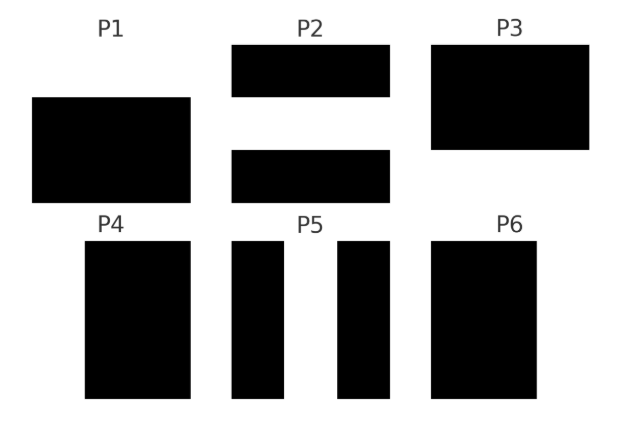
\includegraphics[width=0.6\textwidth]{./figures/question8a.png}
				\caption{الگوهای \(P_1\) تا \(P_6\) به صورت پیکسل‌های سفید و سیاه}
				\label{fig:question8a}
			\end{figure}
			
			\part[ب]
			طراحی یک پرسپترون تک‌لایه با یک نورون برای جدا کردن این الگوها:
			
			\begin{itemize}
				\item وزن‌ها و بایاس اولیه:
				\[
				w_1 = w_2 = \cdots = w_9 = 0,\quad b = 0.
				\]
				\item تابع فعال‌سازی: 
				\(\displaystyle
				y = \mathrm{sign}\bigl(\mathbf{w}^\top \mathbf{x} + b\bigr)
				\in\{+1,-1\}.
				\)
				\item قانون یادگیری پرسپترون:
				\[
				w_i \leftarrow w_i + \eta\,(d - y)\,x_i,
				\quad
				b \leftarrow b + \eta\,(d - y),
				\]
				که \(\eta\) نرخ یادگیری، \(d\) برچسب هدف و \(x_i\) مؤلفهٔ \(i\)ام ورودی است.
			\end{itemize}
			
			\lstinputlisting[language=Python, caption=پیاده‌سازی پرسپترون برای سوال ۸]{./scripts/perceptron8.py}
			
			در پایان آموزش تا همگرایی، وزن‌ها و بایاس نهایی به صورت زیر به دست می‌آیند:
			\[
			\mathbf{w}_{\mathrm{final}} = [\,w_1^*, w_2^*, \dots, w_9^*\,],
			\quad
			b_{\mathrm{final}} = b^*.
			\]
			
		\end{parts}
		
	\end{questions}
	
\end{document}
